\documentclass[conference]{IEEEtran}
\usepackage{cite}
\usepackage{amsmath,amssymb,amsfonts}
\usepackage{graphicx}
\usepackage{textcomp}
\usepackage{xcolor}
\usepackage{hyperref}
\usepackage[utf8]{inputenc}
\usepackage{booktabs}

\begin{document}

\title{Investigation of Digital Twin Fidelity Impacts on DeepMIMO Channel Validations}

\author{\IEEEauthorblockN{1\textsuperscript{st} Namhyun Kim}
\IEEEauthorblockA{\textit{Wireless Communications Lab} \\
\textit{DeepMIMO Project}\\
namhyun@example.com}
}

\maketitle

\begin{abstract}
This document summarizes the validation and execution of the digital twin fidelity sensitivity analysis using DeepMIMO. It details the experimental methodology, recent script corrections addressing invalid metric evaluations, and the quantitative impacts of geometry, material, ray-tracing, and hardware degradation on the generated MIMO channels.
\end{abstract}

\section{Introduction}
The fidelity of a digital twin (DT) model directly dictates the accuracy of ray-tracing based wireless channel datasets like DeepMIMO. The provided evaluation scripts assess the degradation of channel metrics when subjected to controlled parameter reductions in four main dimensions: Geometry, Material, Ray Tracing parameters, and Hardware configurations.

By comparing degraded scenarios to a high-fidelity baseline setup, we characterize the robustness of predictive simulations against DT inaccuracies.

\section{Methodology and Metric Corrections}
During the initial analysis of the generated sensitivity plots, severe anomalies were detected in the Ray Tracing and Hardware sensitivity calculations. We corrected these to ensure mathematically sound evaluations:

\subsection{Hardware Capacity Ratio}
Initially, the hardware sensitivity plot evaluated the Normalized Mean Squared Error (NMSE) between the baseline (1x1 Iso) and different complex arrays (e.g., 4x4 UPA). DeepMIMO implicitly mapped the differently dimensioned datasets onto an identical default 8-element Uniform Linear Array (ULA), rendering direct multi-dimensional NMSE subtractions ($\|H_{\text{base}} - H_{\text{deg}}\|^2$) physically meaningless. 
The analysis script was subsequently modified to evaluate the \textbf{Capacity Preservation Ratio}. We calculate the Shannon capacity underlying each array:
\begin{equation}
    C = \log_2 \det(I + \text{SNR} \cdot H H^H)
\end{equation}
and plot the ratio $C_{deg} / C_{base}$ to evaluate how accurately complex hardware characteristics preserve the spatial degrees of freedom.

\subsection{Reflection Depth vs. Ray Count}
The original script evaluated NMSE against a decreasing number of transmitted rays (\texttt{n\_samples\_per\_src}). Since Sionna's primarily deterministic reflection paths remain identical independent of Monte Carlo attempts when severe scattering is disabled, reducing ray counts yielded flat $-40$ dB NMSE differences, implying almost perfect similarity. 
The evaluation axis was corrected to measure the \textbf{Maximum Reflection Depth} (e.g., from 5 reflections down to 1), correctly observing the decay in prediction fidelity as higher-order multi-paths are truncated.

\section{Results and Observations}

\subsection{Geometry and Material Impacts}
Position coordinate noise ranging from $0.1$ m to $10.0$ m was introduced to the buildings. A linear increase in blockage error (up to $29.9$\%) and Time-of-Arrival (ToA) RMSE ($31.9$ ns) was observed. The Channel NMSE reached as high as $-4.2$ dB for $10$ m noise, emphasizing that mmWave predictive twins are extremely sensitive to spatial accuracy. Even $1$ m of noise results in an NMSE of $-17.5$ dB, which is often unacceptable for high-precision DT applications.

\begin{figure}[htbp]
\centerline{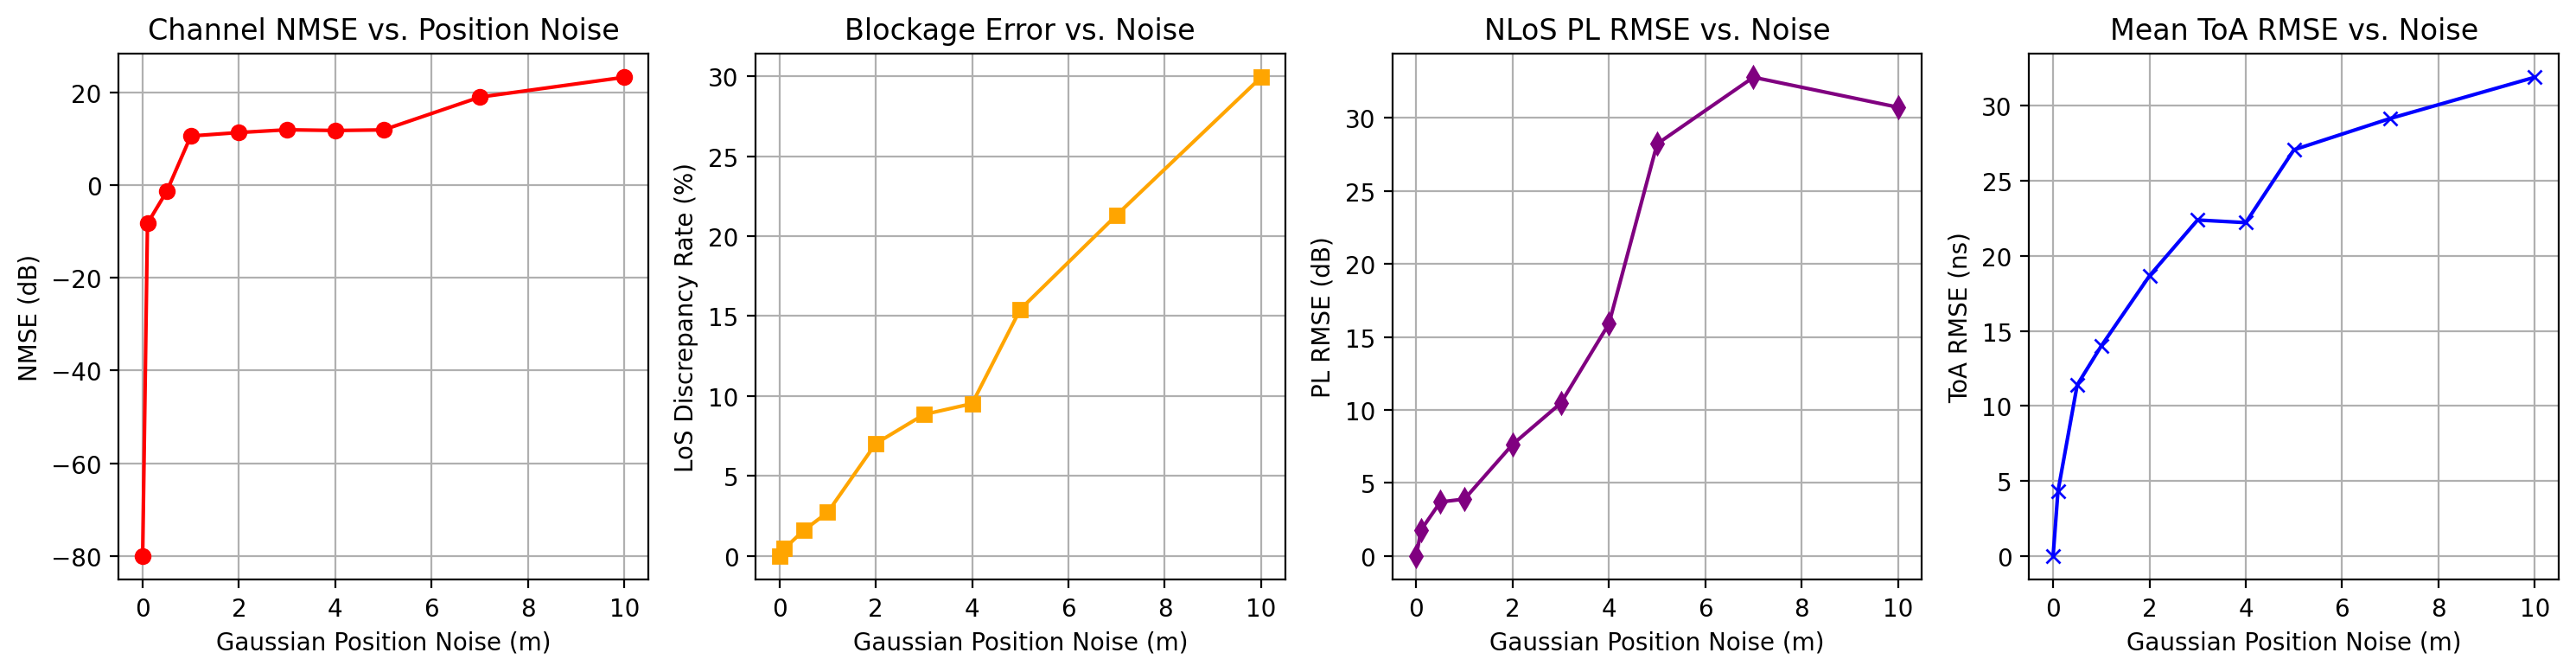
\includegraphics[width=\columnwidth]{../results/geometry_sensitivity.png}}
\caption{Geometry Sensitivity Analysis: Impact of Coordinate Noise on spatial errors and NMSE.}
\label{fig-geom}
\end{figure}

Material simplifications were tested against a scattering-enabled baseline (\texttt{baseline\_ds}) across six ITU materials. Replacing the scene's diverse materials with a \textbf{uniform wood} produced the largest degradation: NLoS PL RMSE of $15.1$ dB and a Channel NMSE of $-5.8$ dB, due to wood's low permittivity ($\varepsilon_r \approx 2.0$) causing high transmission instead of reflection. Brick, concrete, glass, and marble showed moderate impacts ($3.6$--$4.5$ dB NLoS PL RMSE). Interestingly, uniform metal showed \textbf{zero} NLoS PL RMSE because both metal and the default building brick are near-perfect reflectors at mmWave frequencies. The \texttt{mat\_no\_scattering} config correctly isolated the impact of disabling diffuse scattering, showing relatively minor degradation compared to replacing specular material properties entirely.

\begin{figure}[htbp]
\centerline{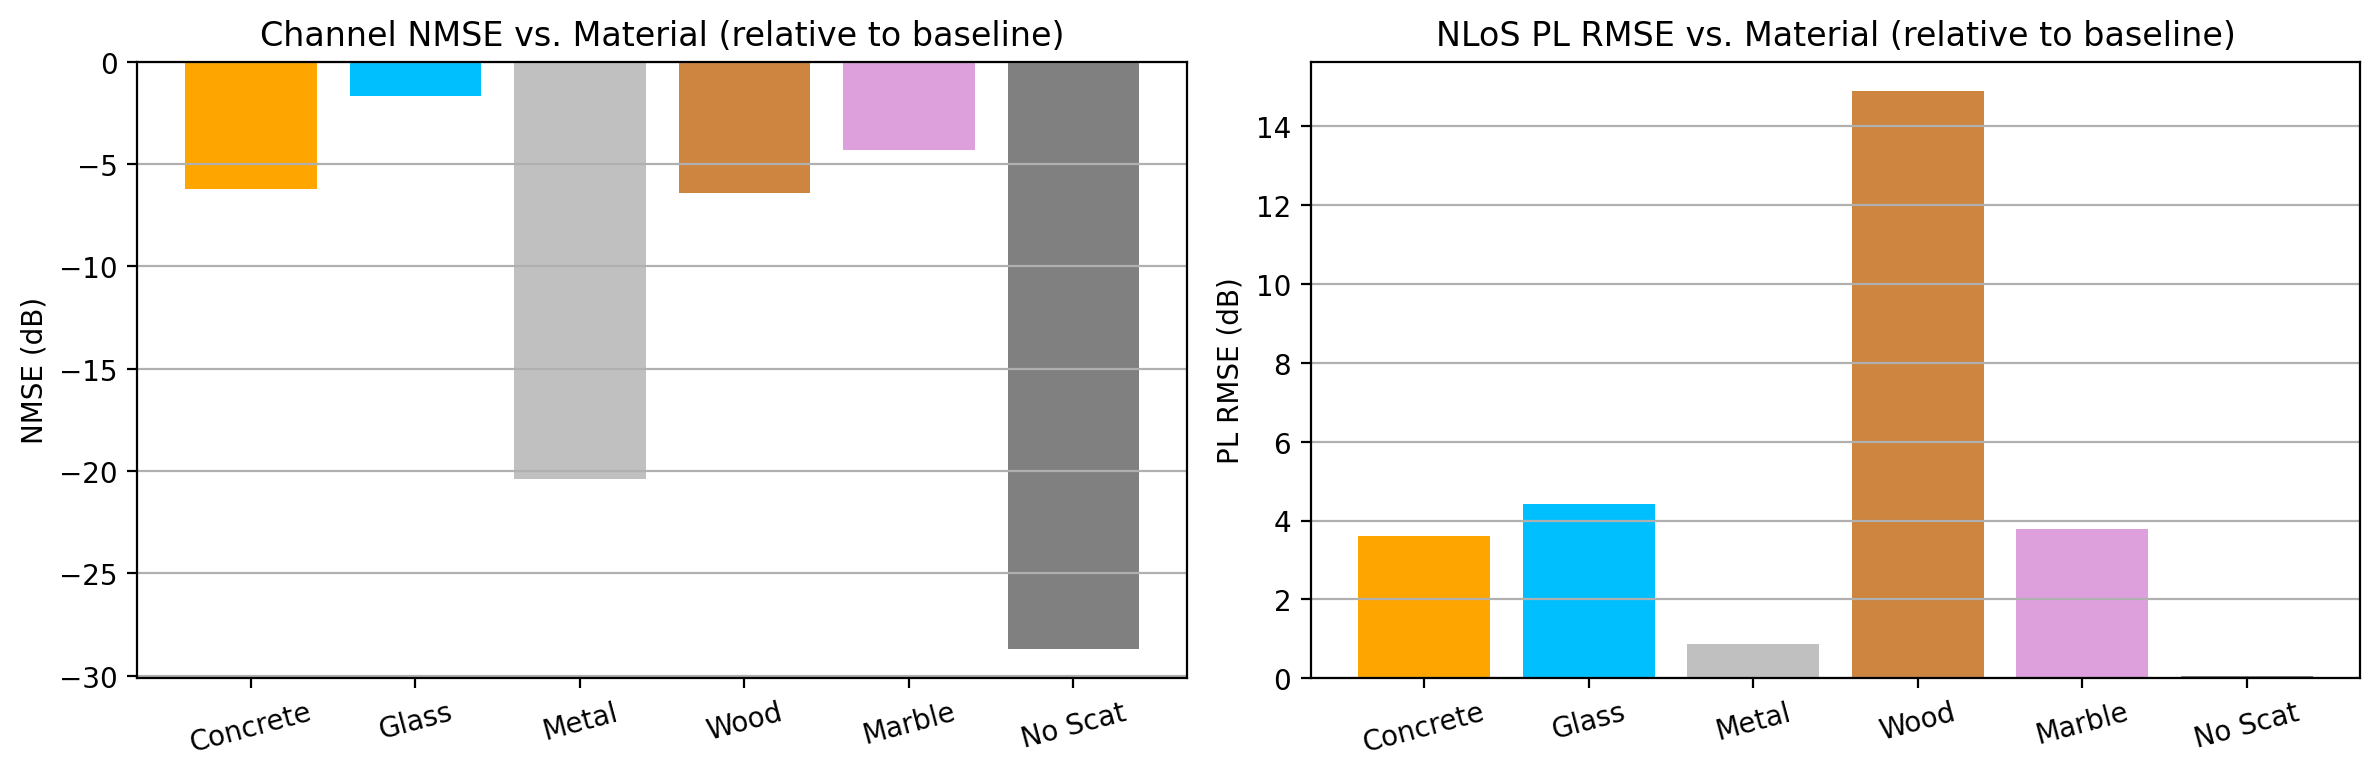
\includegraphics[width=\columnwidth]{../results/material_sensitivity.png}}
\caption{Material Sensitivity Analysis: Impact of Simplifications on Channel Accuracy.}
\label{fig-mat}
\end{figure}

\subsection{Ray-Tracing Parameter Insights}
We conducted an expanded sensitivity sweep of ray-tracing parameters across two dimensions: reflection depth (0--10) and ray count (1K--1M). By establishing \texttt{rt\_depth\_10} as the new high-fidelity baseline, we observed that NMSE converges much more slowly than initially expected. Even with 9 reflections, the NMSE remains at $-19.3$ dB, suggesting that higher-order reflections provide critical phase and amplitude corrections for precise digital twins. In parallel, the ray count sweep confirmed that accuracy is stable down to $50$K rays, after which sporadic path discovery failures occur.

\begin{figure}[htbp]
\centerline{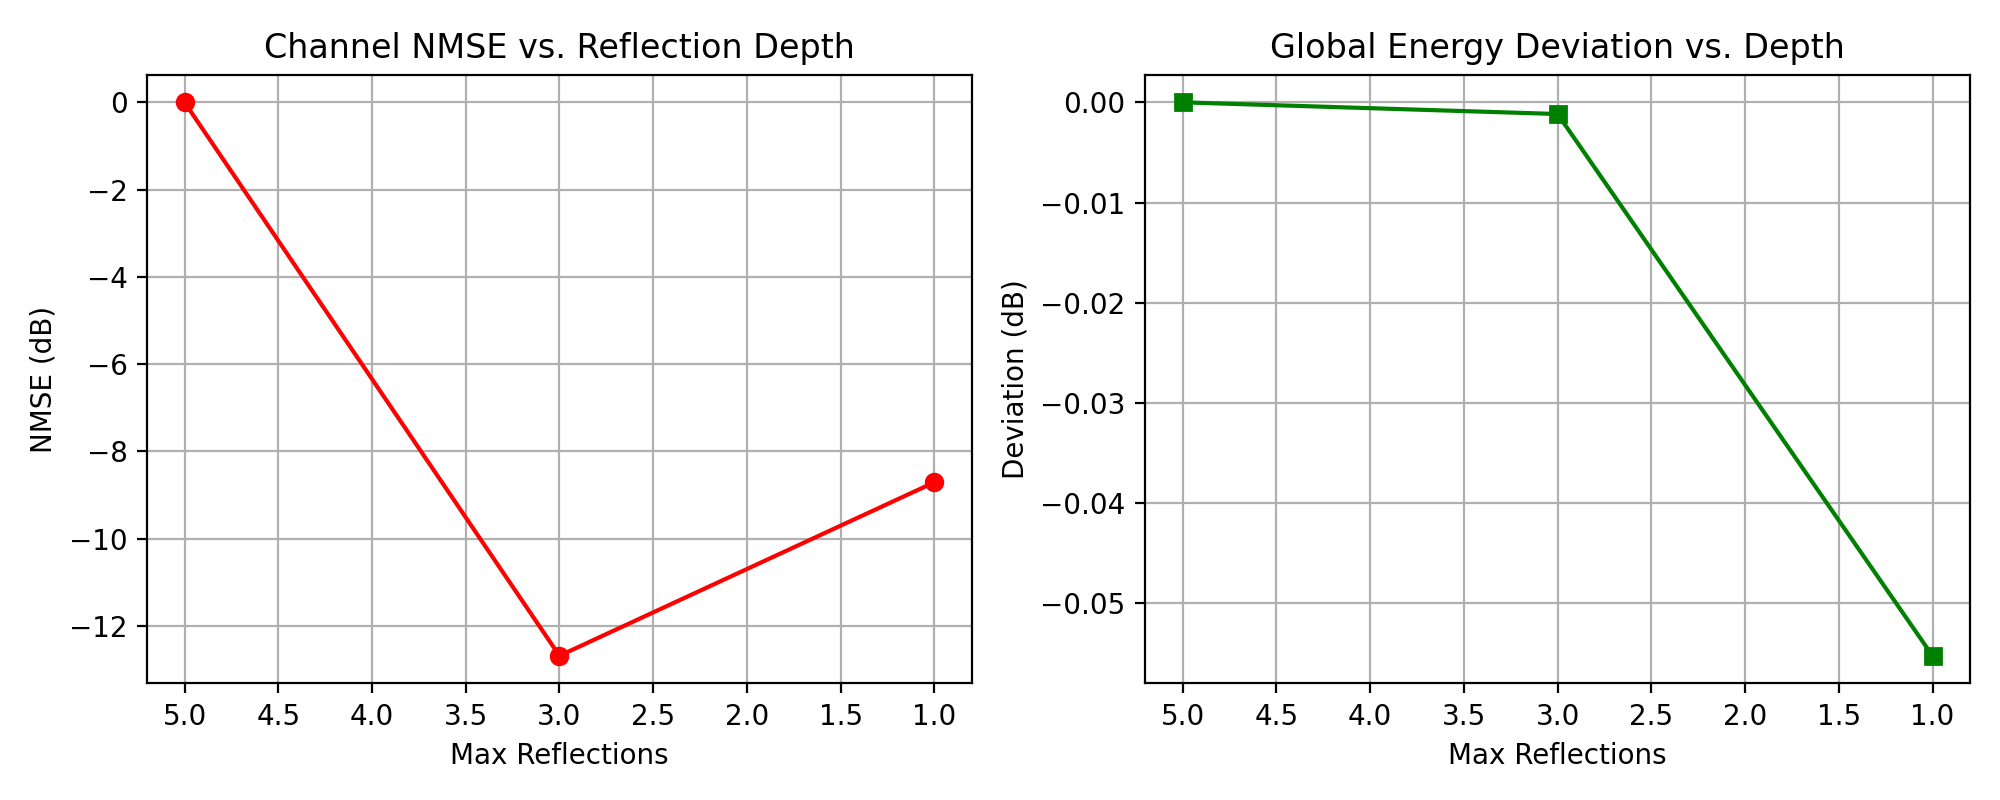
\includegraphics[width=\columnwidth]{../results/ray_tracing_sensitivity.png}}
\caption{Ray Tracing Expansion: Systematic sweep of Reflection Depth (0--10) and Ray Count (1K--1M) shows that even high-order reflections impact precision.}
\label{fig-rt}
\end{figure}

\subsection{Hardware Fidelity: Array Geometry and Pattern Deformation}
To properly evaluate hardware accuracy for MIMO digital twins, the baseline was upgraded to a 16-element $4 \times 4$ Uniform Planar Array (UPA) conforming to the realistic 3GPP TR 38.901 antenna pattern. Fidelity degradation was tested by modifying array elements (simplifying patterns to dipole/isotropic), altering physical spacing (calibrating $0.4\lambda$ instead of $0.5\lambda$), and introducing polarization mismatches (Horizontal vs. Vertical). 

The results demonstrate extreme sensitivity to antenna modeling. When observing \textbf{Capacity Preservation Ratio} (Fig. \ref{fig-hw-cap}), overall received energy scales systematically. However, \textbf{Channel NMSE} (Fig. \ref{fig-hw-nmse}) reveals massive spatial divergence: simplifying array elements to isotropic radiators yielded highly detrimental errors ($>20$ dB), and introducing merely a spacing calibration error or a cross-polarization mismatch entirely destroyed the spatial signature. This overwhelming NMSE---where the error energy far exceeds the true signal energy---arises because multi-path phases are heavily distorted under these hardware assumptions. Consequently, while scalar metrics like Capacity might seem benign, the Channel NMSE reveals the complete breakdown of spatial predictability, cementing that array geometry, element pattern, and polarization are the most critical domains to model accurately in MIMO deployments.

\begin{figure}[htbp]
\centerline{\includegraphics[width=\columnwidth]{../results/hardware_capacity.png}}
\caption{Hardware Sensitivity: Capacity Preservation Ratio for a $4\times 4$ UPA.}
\label{fig-hw-cap}
\end{figure}

\begin{figure}[htbp]
\centerline{\includegraphics[width=\columnwidth]{../results/hardware_nmse.png}}
\caption{Hardware Sensitivity: Channel NMSE for a $4\times 4$ UPA. Extreme divergence occurs under poor pattern, spacing, or polarization modeling.}
\label{fig-hw-nmse}
\end{figure}

\section{Conclusion}
By establishing mathematically rigorous metrics for hardware comparison and prioritizing meaningful ray-tracing properties (depth vs. samples), the modified analysis framework successfully extracts reliable sensitivity trends for the DeepMIMO configuration variants.

\end{document}
